\section{Ultrasound on objects}
\begin{figure}[h]
    \centering
    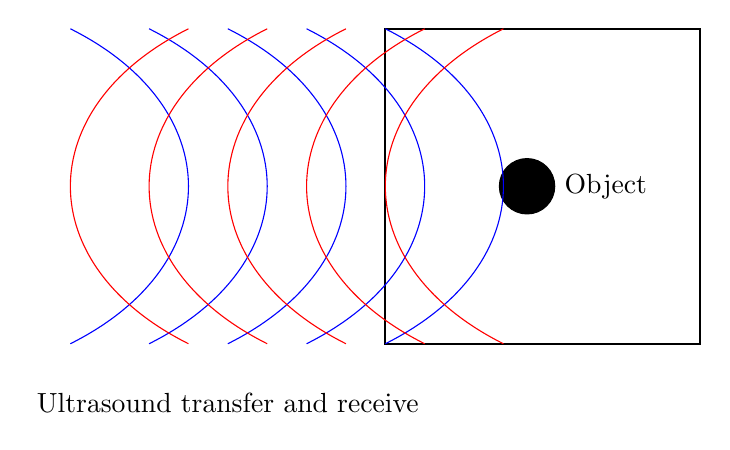
\begin{tikzpicture}
    \filldraw[color=black] (-2.2,0) circle (10pt) node[xshift=1cm] {Object};
    \draw[thick] (-4,-2) rectangle (0,2);
    \foreach \x in {4,5,6,7,8}
        \draw[color=blue] (-\x,2) .. controls (-\x+2,1) and (-\x+2,-1) .. (-\x,-2);
    \foreach \x in {2.5,3.5,4.5,5.5,6.5}
        \draw[color=red] (-\x,2) .. controls (-\x-2,1) and (-\x-2,-1) .. (-\x,-2);
    \draw (-6,-2.5) node[anchor=north] {Ultrasound transfer and receive};
    \end{tikzpicture}
    \caption{Ultrasound}
    \label{fig:Ultrasound}
\end{figure}